\documentclass[11pt,a4paper]{article}

% PACKAGES
\usepackage[utf8]{inputenc}
\usepackage[T1]{fontenc}
\usepackage[slovak]{babel}
\usepackage{amsmath, amssymb}
\usepackage{amsthm} % For theorem environments
\usepackage{graphicx}
\usepackage{enumerate}
\usepackage{tikz}
\usetikzlibrary{tikzmark}
\usepackage[all,pdf,2cell]{xy}
\usepackage{soul}
\usepackage{framed}

% THEOREM ENVIRONMENTS SETUP
% Style for definitions and examples (upright text, bold title)
\theoremstyle{definition} 
\newtheorem{definition}{Definícia}[section]
\newtheorem{example}[definition]{Príklad}

% Style for theorems (italicized text, bold title)
\theoremstyle{plain} 
\newtheorem{tvrdenie}[definition]{Tvrdenie}
\newtheorem{veta}[definition]{Veta}

% Style for remarks and questions (upright text, italic title)
\theoremstyle{remark} 
\newtheorem*{question}{Otázka}

% Macros

% Simple abbreviations
\newcommand{\id}{\mathrm{id}}
\newcommand{\Nat}{\mathbb{N}}
\newcommand{\Set}{\mathbf{Set}}
\newcommand{\R}{\mathbb{R}}

% More complex stuff
% Restriction of a function (from stackexchange)
\newcommand\restr[2]{{% we make the whole thing an ordinary symbol
  \left.\kern-\nulldelimiterspace % automatically resize the bar with \right
  #1 % the function
  \littletaller % pretend it's a little taller at normal size
  \right|_{#2} % this is the delimiter
  }}
\newcommand{\littletaller}{\mathchoice{\vphantom{\big|}}{}{}{}}

% DOCUMENT START
\begin{document}
\title{Lineárna algebra 1\\(texty k prednáškam)}
\author{Gejza Jenča}
\date{Verzia 1}
\maketitle
\section{Množiny}

\begin{definition}[Množina]\label{def:mnozina}
\emph{Množina} je súbor objektov, nazývaných \emph{prvkami množiny}.
Fakt, že objekt $x$ je prvkom množiny $A$ značíme takto:
$$x \in A$$
Ak objekt $x$ nepatrí do množiny $A$, značíme to takto:
$$x \notin A$$
\end{definition}

Množiny môžu byť konečné alebo nekonečné.
Konečnú množinu môžeme špecifikovať prostým vymenovaním jej prvkov takto:
$$A = \{1, \text{slon}, \{2\}\}$$
Platí $1 \in A$, slon $\in$ $A$.
Zrejme $4 \notin A$ mačka $\notin$ $A$.

\begin{question}
Platí $2 \in A$?
Odpoveď: nie.
\end{question}

Ale ak si niekto myslí, že áno, musí si myslieť, že objekt 2 je rovný niektorému z objektov, ktoré patria do množiny $A$.
Pravdepodobne si myslí, že
$$2 = \{2\}$$
To však nie je pravda: 2 nie je množina a \{2\} je množina a teda tieto dva objekty nemôžu byť rovné, pretože rovnaké objekty majú rovnaké vlastnosti.
Príkladom nekonečnej množiny je množina všetkých prirodzených čísel
$$\mathbb{N}=\{0,1,2,3,4,...\}$$
Všimnime si, že $0 \in \mathbb{N}$;
je možné, že na iných prednáškach to bude konvencia $0 \notin \mathbb{N}$.
Ďalšie množiny čísel, ktoré poznáte zo strednej školy, sú:
\begin{itemize}
    \item množina všetkých celých čísiel $\mathbb{Z}$
    \item množina všetkých racionálnych čísel $\mathbb{Q}$
    \item množina všetkých reálnych čísel $\mathbb{R}$.
\end{itemize}

\begin{definition}[Prázdna množina]
\emph{Prázdna množina} je množina, ktorá neobsahuje žiadny objekt. Prázdnu množinu značíme $\emptyset$.
\end{definition}

\begin{definition}[Podmnožina]
Hovoríme, že množina $B$ je \emph{podmnožinou} množiny $A$, ak pre každý prvok $x$ množiny $B$ platí, že $x \in A$.
Fakt, že $B$ je podmnožinou $A$ značíme
$$B \subseteq A$$
Ak $B$ nie je podmnožinou $A$, značíme $B \not\subseteq A$.
Vzťah $B \subseteq A$ sa volá \emph{inklúzia}.
\end{definition}

\noindent\textbf{Príklady:}
\begin{itemize}
    \item $A=\{1, \text{slon}, \{2\}\}$, potom
    \item $\{1, \text{slon}\} \subseteq A$
    \item $\{1, \{2\}\} \subseteq A$
    \item $\{1,3\} \not\subseteq A$, lebo $3 \in \{1,3\}$ a zároveň $3 \notin A$
    \item $\{2\} \not\subseteq A$, lebo $2 \in \{2\}$ a zároveň $2 \notin A$
\end{itemize}

\noindent V jazyku formálnej logiky $B \subseteq A$ zapisujeme takto:
%$$ (\forall x), x \in B \Rightarrow x \in A $$
%Pre všetky $x$ platí, že ak $x$ patrí do $B$, potom $x$ patrí do $A$.
\begin{center}
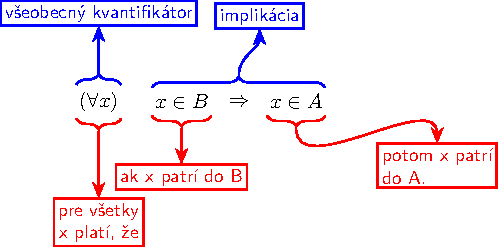
\includegraphics{figures/predn1_fig1.pdf}
\end{center}
\noindent Iný spôsob čítania tej istej formuly je tento:
%$$ (\forall x \in B), x \in A $$
%Pre všetky $x$ z množiny $B$ platí, že $x$ patrí do $A$.
\begin{center}
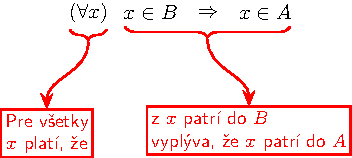
\includegraphics{figures/predn1_fig2.pdf}
\end{center}
Iný spôsob zápisu $B\subseteq A$ je tento
\begin{center}
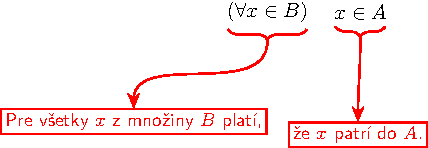
\includegraphics{figures/predn1_fig3.pdf}
\end{center}
Tieto symbolické zápisy sú logicky ekvivalentné, teda vyjadrujú rovnaký vzťah medzi množinami $B$ a $A$.
V tejto chvíli je dobré uvedomiť si, že prázdna množina je podmnožinou každej množiny.
Naozaj, ak by pre nejakú množinu $A$ platilo $\emptyset \not\subseteq A$, musel by existovať prvok $x$ množiny $\emptyset$ taký, že $x$ nepatrí do $A$.
Inak povedané, malo by platiť $x \in \emptyset$ a zároveň $x \notin A$;
to však nie je možné, pretože $x \in \emptyset$ neplatí pre žiadny objekt $x$.
Pri úvahách o vzťahu "byť podmnožinou" sme vlastne používali toto tvrdenie:

\begin{veta}
Nech $A, B$ sú množiny.
Potom $B \not\subseteq A$ práve vtedy, keď existuje $x \in B$ také, že $x \notin A$.
\end{veta}

\noindent V jazyku formálnej logiky:
%$$ (\exists x), x \in B \land x \notin A $$
%Existuje také $x$, že $x$ patrí do $B$ a zároveň $x$ nepatrí do $A$.
\begin{center}
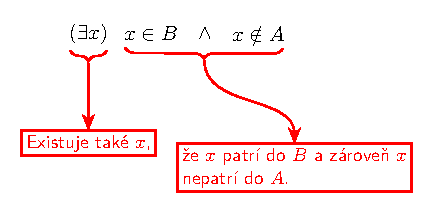
\includegraphics{figures/predn1_fig4.pdf}
\end{center}
Kedy sú dve množiny rovné?
Keďže množina je súbor objektov do nej patriacich, dve množiny sú rovné, ak obsahujú rovnaké prvky:
$$A = B \text{ práve vtedy, keď pre všetky objekty } x \text{ platí, že } x \in A \text{ práve vtedy, keď } x \in B.$$
Táto vlastnosť množín sa volá extenzionalita.
Z toho vyplýva nasledujúce tvrdenie:

\begin{veta}
Nech $A, B$ sú množiny. Potom $A=B$ práve vtedy, keď $A \subseteq B$ a zároveň $B \subseteq A$.
\end{veta}

Jeden zo spôsobov ako môžeme špecifikovať množinu je vydelenie z nejakej množiny pomocou výroku o prvkoch:
$$ \{x \in A \mid \text{výrok o } x\} $$
\textbf{Príklady:}
\begin{itemize}
    \item $\{x \in \mathbb{R} \mid x \ge 2\} = \langle 2, \infty)$
    \item $\{x \in \mathbb{R} \mid x > 3\} = (3, \infty)$
    \item $\{x \in \mathbb{R} \mid x \ge 4 \text{ a zároveň } x < 100\} = \langle 4, 100)$
    \item $\{x \in \mathbb{R} \mid x \ge 3 \text{ a zároveň } x < 2\} = \emptyset$
    \item $\{x \in \mathbb{R} \mid x^2 = 2\} = \{\sqrt{2}, -\sqrt{2}\}$
    \item $\{x \in \mathbb{N} \mid x^2 = 2\} = \emptyset$
    \item $\{n \in \mathbb{N} \mid (n+1) \text{ je prvočíslo}\} = \{1, 2, 4, 6, ...\}$
\end{itemize}

Podobný (ale významovo odlišný) zápis je
$$ \{ \text{výraz závislý od } x \mid x \in A \} $$
\textbf{Príklady:}
\begin{itemize}
    \item $\{n^2 \mid n \in \mathbb{N}\} = \{0, 1, 4, 9, 16, ...\}$
    \item $\{\sin(x) \mid x \in \mathbb{R}\} = \langle -1, 1 \rangle$
\end{itemize}

\subsection{Kardinalita množiny}
Počet prvkov konečnej množiny $A$ sa volá kardinalita $A$ a označujeme $|A|$.
\noindent\textbf{Príklady:}
\begin{itemize}
    \item $|\{1,7,8\}|=3$
    \item $|\emptyset|=0$
    \item $|\{\{4'4,2,3\}\}|= 1$
    \item $|\{\emptyset\}|=1$
\end{itemize}

\subsection{Operácie na množinách}
Ak $A, B$ sú množiny môžeme z nich vytvoriť inú množinu pomocou množinových operácií.
\begin{align*}
    A \cup B &= \{x \mid x \in A \text{ alebo } x \in B\} \quad \text{(zjednotenie množín A, B)} \\
    A \cap B &= \{x \mid x \in A \text{ a zároveň } x \in B\} \quad \text{(prienik množín A, B)} \\
    A \setminus B &= \{x \in A \mid x \notin B\} \quad \text{(rozdiel množín)}
\end{align*}

\noindent\textbf{Príklady:}
\begin{itemize}
    \item $\{1,2,3\} \cup \{2,3,4\} = \{1,2,3,4\}$
    \item $\{1,2,3\} \cap \{2,3,4\} = \{2,3\}$
    \item $\langle 2,4 \rangle \cap \langle 3,5 \rangle = \langle 3,4 \rangle$
    \item $\langle 2,3 \rangle \cap \langle 3,5 \rangle = \emptyset$
    \item $\langle 2,4 \rangle \cup \langle 3,5 \rangle = \langle 2,5 \rangle$
    \item $A \cap A = A \cup A = A$, pre všetky množiny $A$
    \item $\{1,2,3\} \setminus \{2,3,4\} = \{1\}$
    \item $\langle 2,4 \rangle \setminus \langle 3,5 \rangle = \langle 2,3)$
    \item $\mathbb{R} \setminus \mathbb{Q} = \text{iracionálne čísla}$
    \item $A \setminus A = \emptyset$, pre všetky množiny $A$
\end{itemize}

\subsection{Kartézsky/Priamy súčin množín}
Ak $a, b$ sú nejaké objekty, môžeme z nich vytvoriť objekt zvaný usporiadaná dvojica $(a, b)$. Dôležité je, že $(a,b) \neq (b,a)$, ak $a \neq b$.
V dvojici $(a,b)$, $a$ je prvá zložka a $b$ je druhá zložka.

\begin{definition}[Kartézsky súčin]
Nech $A, B$ sú množiny.
\emph{Kartézsky súčin} $A \times B$ je množina všetkých usporiadaných dvojíc $(a, b)$, kde $a \in A$ a $b \in B$.
Symbolicky: $A \times B = \{(a,b) \mid a \in A, b \in B\}$.
\end{definition}

\noindent\textbf{Príklady:}
\begin{itemize}
    \item $\{1,2\} \times \{3,4\} = \{(1,3), (1,4), (2,3), (2,4)\}$
    \item $\{1\} \times \{\square, \oplus\} = \{(1,\square), (1,\oplus)\}$
    \item $\{3,4\} \times \{1,2\} = \{(3,1), (3,2), (4,1), (4,2)\}$
\end{itemize}
Vidíme, že vo všeobecnosti nie je pravda, že $A \times B = B \times A$.
\begin{question}
Čo je $A \times \emptyset$?
\end{question}
$$ A \times \emptyset = \{(a,b) \mid a \in A, b \in \emptyset\} $$
Taký objekt $b$ neexistuje!
Teda $A \times \emptyset = \emptyset$ pre každú množinu $A$.
Nič nám nebráni vytvoriť kartézsky súčin $A \times A$: ak $A=\{1,2\}$, potom
$$A \times A = \{(1,1), (1,2), (2,1), (2,2)\}$$
Toto sa označuje aj $A^2$ -- druhá kartézska mocnina.
Analogicky ako pojem usporiadanej dvojice môžeme vytvoriť pojem usporiadanej trojice,
štvorice, $n$-tice, $n \in \mathbb{N}$.
\[
(a,b,c)\quad(a,b,c,d)\quad(a_1,\dots,a_n)
\]
Neformálne budeme na prednáškach používať
neexistujúce slovenské slovo ,,tica'' ak budem chcieť vyjadriť, že niečo je dvojica,
trojica, ..., ale pritom mi je jedno koľko zložiek má.
Toto je pokusom anglického
slova \emph{tuple}.
Pojem kartézskeho súčinu dvoch množín môžeme rozšíriť analogicky na viac množín:
\begin{align*}
    A \times B \times C &= \{(a,b,c) \mid a \in A, b \in B, c \in C\} \\
    A \times B \times C \times D &= \{(a,b,c,d) \mid a \in A, b \in B, c \in C, d \in D\}
\end{align*}
Na tomto predmete nás budú najmä zaujímať tieto množiny:
\begin{itemize}
    \item $\mathbb{R}^1 = \mathbb{R}$
    \item $\mathbb{R}^2 = \mathbb{R} \times \mathbb{R}$
    \item $\mathbb{R}^3 = \mathbb{R} \times \mathbb{R} \times \mathbb{R}$
    \item $\mathbb{R}^n = \underbrace{\mathbb{R} \times \mathbb{R} \times \dots \times \mathbb{R}}_{n\text{-krát}}$ (všetky usporiadané n-tice reálnych čísel)
\end{itemize}
Pr.
$(1, \sqrt{2}, -\pi, 17) \in \mathbb{R}^4$.




\section{Zobrazenia}

Zobrazenia sa často nazývajú funkcie. Obe slová znamenajú to isté, obvykle však funkcia zobrazuje do čísel ($\mathbb{N}, \mathbb{R}, \mathbb{C}, \dots$).
Ktoré slovo sa použije je otázkou konvencie v danej časti matematiky.

\begin{definition}[zobrazenie]\label{def:zobrazenie}
Nech $A, B$ sú množiny.
\emph{Zobrazenie} $f$ z $A$ do $B$ je predpis, ktorý každému prvku
$A$ priradí nejaký prvok $B$.
Zapisujeme 
\[
f \colon A \to B.
\]
$A$ je \emph{definičný obor}, $B$ je \emph{koobor}.
\end{definition}

To znamená, že ak chceme špecifikovať nejaké zobrazenie $f$, musíme špecifikovať tri
veci:
\begin{enumerate}
    \item Z ktorej množiny sa zobrazuje (definičný obor).
    \item Do ktorej množiny sa zobrazuje (koobor).
    \item Predpis, ktorý nám určí, pre každý prvok definičného oboru ktorý prvok sa mu má zobraziť.
\end{enumerate}

Predpis môže byť daný rôzne.
Napríklad ak $f \colon \mathbb{R} \to \mathbb{R}$ môžeme predpis niekedy poznamenať pomocou vzorca, napr.
\[
f(x) = \sqrt{x^2+1}
\]
Ale $A, B$ vôbec nemusia byť množiny čísel, a predpis nemusí byť vzorec!
\begin{example}
Niekedy $A$ nemá číselnú povahu, $B$ áno.
\begin{itemize}
    \item $A = \text{všetky adresy v meste}$
    \item $B = \mathbb{R}$
\end{itemize}
Zobrazenie $d \colon A \to B$ môže byť \[
d(x) = \text{najkratšia vzdialenosť pri ceste peši medzi adresou $x$ a SvF STU, v minútach}.\]
Napríklad: $d(\text{moje bydlisko}) = 80$, $d(\text{Bernolákova 1})=8$.
\end{example}


\begin{example}
$g \colon \mathbb{N} \rightarrow \mathbb{N}$ dané predpisom $g(n) = n^2 + 1$.
Toto nám hovorí, že $g$ zobrazuje z množiny všetkých prirodzených čísel do množiny všetkých prirodzených čísel.
Predpis je teda v tomto prípade daný vzorcom, ktorý nám umožňuje počítať hodnoty zobrazenia pre konkrétne prvky definičného oboru $g$ (t.j. prirodzené čísla) dosadením a výpočtom.
\begin{align*}
    g(2) &= 2^2 + 1 = 5 \\
    g(7) &= 7^2 + 1 = 50
\end{align*}
$g(-1) = ?$ Toto neexistuje, pretože $-1 \notin \mathbb{N}$ a nie je to teda prvok definičného oboru $g$.
\end{example}

\begin{example}\label{ex:jedlo}
Nech $A = \{\text{Jožko, Miško}\}$ a $B = \{\text{bageta, guláš, jablko}\}$.
Nech $j \colon A \rightarrow B$ je zobrazenie "najobľúbenejšie jedlo".
V tomto prípade je definičný konečná množina.
Preto nám stačí napísať hodnotu
zobrazenia $j$ v každom prvku množiny $A$:
\begin{itemize}
    \item $f(\text{Jožko}) = \text{bageta}$
    \item $f(\text{Miško}) = \text{guláš}$
    \item $f(\text{Janka}) = \text{guláš}$
\end{itemize}

Zobrazenie $j$ môžeme aj nakresliť:
\begin{center}
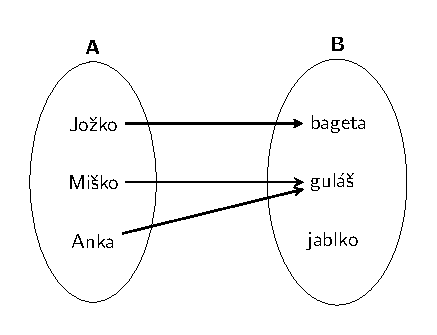
\includegraphics{figures/predn2_fig1.pdf}
\end{center}
\end{example}

Iný spôsob špecifikácie predpisu zobrazenia je napríklad tabuľkou:
\begin{center}
\begin{tabular}{c|ccc}
    $x$ & Jožko & Miško & Anka \\
    \hline
    $j(x)$ & bageta & guláš & guláš
\end{tabular}
\end{center}
Tu sa, samozrejme, nesmú prvky v hornom riadku opakovať.
\begin{example}
Nech $H$ je množina všetkých ľudí (aj z minulosti).
$\sigma \colon H \rightarrow H$ je zobrazenie dané predpisom $\sigma(x) = \text{otec človeka } x$.
\end{example}

\begin{example}
$S$ - množina všetkých občanov SR.
$\eta \colon S \rightarrow \mathbb{N}$ dané predpisom $\eta(x) = \text{rodné číslo}$.
\end{example}

\begin{example}
$B = \{\text{bageta, guláš, jablko}\}$. Nech $k \colon B \rightarrow \mathbb{R}$ je zobrazenie "koľko kalórií".
Keďže $B$ je konečná, stačí nám napísať:
$k(\text{guláš}) = 677$, $k(\text{bageta}) = 1148$, $k(\text{jablko}) = 301.4$.
\end{example}

\begin{example}
Poznáme nejaký príklad zobrazenia typu $A\times A\to A$, kde $A$ je nejaká množina? Samozrejme, už od prvého ročníka
základnej školy. Vezmime $A=\Nat$; sformulovať nejaký predpis pre zobrazenie 
$\Nat\times\Nat\to\Nat$ znamená povedať, ako vyrobiť z usporiadanej dvojice prirodzených čísel prirodzené
číslo. Napríklad môžeme definovať zobrazenie $+\colon A\times A\to A$ predpisom
\[
+(x,y)=\text{súčet čísel $x,y$}
\]
máme teda $+(1,3)=4$, $+(4,4)=8$. Samozrejme, zaužívaný spôsob zapisovania hodnoty zobrazenia $+$ v nejakej dvojici
$(a,b)\in\Nat\times\Nat$ je iný, nepíšeme obvykle $+(a,b)$, ale znak zobrazenia dáme medzi prvú a druhú zložku
usporiadanej dvojice, $a+b$. To je však detail, ktorý nič nemení na dôležitom náhľade, že sčítanie je zobrazením
z nejakej množiny do inej množiny.
\end{example}

Predošlý príklad je poučný v tom, že ukazuje ako jazyk postavený na pojmoch ,,množina'' a ,,zobrazenie'' umožňuje
popisovať matematické pojmy. Tento jazyk sa začal účinne používať na popis existujúcej a objavovanie novej matematiky v
20. storočí a dnes si už matematiku bez množín ani nevieme predstaviť.

Jeden zo spôsobov zapisovania zobrazení je ,,po prípadoch'', ako v nasledujúcich
dvoch príkladoch.
\begin{example}
\emph{Absolútna hodnota} je zobrazenie $\mathbb R\to\mathbb R$ dané predpisom
\[
|x|=
\begin{cases}
x& x\geq 0\\
-x& x<0
\end{cases}
\]
\end{example}
\begin{example}
\emph{Znamienková funkcia} alebo \emph{signum} je zobrazenie 
$\mathrm{sgn}\colon\R\to\R$ dané predpisom
\[
\mathrm{sgn}(x)=
\begin{cases}
1& x>0\\
0& x=0\\
-1& x<0
\end{cases}
\]
\end{example}

Voči Definícii \ref{def:zobrazenie} by bolo možné vzniesť (z istého hľadiska oprávnene) námietku o nepresnosti; používa nejasné slová ako
"priradí", "predpis".
Námietku je možné vyriešiť takto:

\begin{definition}[formálna definícia zobrazenia]\label{def:zobrazenieFormal}
Nech $A$, $B$ sú množiny.
\emph{Zobrazenie} $f$ z $A$ do $B$ je množina $F \subseteq A \times B$ taká, že pre každé $a \in A$ existuje práve jedno $b \in B$ také, že $(a,b) \in F$.
\end{definition}

$(a,b) \in f$ v zmysle Definície \ref{def:zobrazenieFormal} potom znamená $f(a)=b$ v zmysle Definície
\ref{def:zobrazenie}.
Aj keď je Definícia \ref{def:zobrazenieFormal} presnejšia, v skutočnosti ju bežne nikto nepoužíva, ani nikto bežne
nerozmýšľa o zobrazeniach ako o množinách usporiadaných dvojíc.
Niekedy však takéto presné uvažovanie nutne potrebujeme, a preto je dobré vedieť o existencii tohto pohľadu na pojem zobrazenia.
%\subsection*{Koniec formalistickej odbočky}

\begin{definition}[Obor hodnôt]\label{def:oborHodnot}
Nech $f \colon A \rightarrow B$ je zobrazenie. \emph{Obor hodnôt} je množina
$$ \mathcal{H}(f) = \{f(a) | a \in A\} $$
\end{definition}
Čiže máme $b \in \mathcal{H}(f)$ práve vtedy, keď existuje $a \in A$ také, že $f(a)=b$.
Je dôležité si uvedomiť rozdiel medzi oborom hodnôt a kooborom.
Ak napíšeme napríklad
$f \colon \mathbb{R} \rightarrow \mathbb{R}$ dané predpisom $f(x) = x^2 - x + 1$.
Koobor je $\mathbb{R}$, ale $\mathcal{H}(f) = \langle\frac{3}{4}, \infty\rangle$.
Určiť obor hodnôt zobrazenia môže byť teda ťažké a pre prácu so zobrazením to nemusí
byť nutné.
Čo potrebujeme o zobrazení nutne vedieť je koobor, nie obor hodnôt.
Našťastie, keď sa pred našim duševným zrakom zjaví nejaké zobrazenie, vždy je
vybavené kooborom.
Trochu mätúce môže byť, že koobor sa často neuvádza explicitne a
funkcia sa stotožňuje s predpisom, toto sa bežne bude diať na predmete
\emph{Matematická analýza}.
V tomto (a iných) smere sa konvencie v matematických
oblastiach líšia.
Pre profesionálneho matematika však spravidla nie je problém sa
odlišným konvenciám v prípade potreby prispôsobiť, ak potrebuje pracovať s
matematickou literatúrou a podobne.
\begin{definition}[identické zobrazenie]\label{def:identickeZobrazenie}
Nech $A$ je množina. \emph{Identické zobrazenie} (na $A$) je zobrazenie $\id_A \colon A \rightarrow A$ dané predpisom $\id_A(a) = a$, pre každý prvok $a \in A$.
\end{definition}

\begin{definition}[rovnosť zobrazení]\label{def:rovnostZobrazeni}
Nech $A, B, C, D$ sú množiny, nech $f \colon A \rightarrow B$ a $g \colon C \rightarrow D$.
Hovoríme, že $f$ je \emph{rovné} $g$, ak $A=C$, $B=D$ a pre všetky $x \in A=C$ platí, že $f(x)=g(x)$.
\end{definition}

Na lineárnej algebre budeme ohľadom pojmu rovnosti zobrazení trochu striktnejší ako
na iných predmetoch, budeme aplikovať definíciu \ref{def:rovnostZobrazeni} veľmi
presne.
Ilustruje to nasledujúci príklad.

\begin{example}\label{ex:rovnostZobrazeni}
~\par
\begin{enumerate}
    \item[A)] $f \colon \mathbb{Z} \rightarrow \mathbb{N}$ dané predpisom $f(k) = \sqrt{k^2}$ \\
    $g \colon \mathbb{Z} \rightarrow \mathbb{N}$ dané predpisom $g(k) = |k|$ \\
    Platí $f=g$.
    \item[B)] $f \colon \mathbb{N} \rightarrow \mathbb{N}$ dané predpisom $f(k) = \sqrt{k^2}$ \\
    $g \colon \mathbb{N} \rightarrow \mathbb{N}$ dané predpisom $g(k) = |k|$ \\
    Platí $f=g$.
    \item[C)] $f \colon \mathbb{Z} \rightarrow \mathbb{Z}$ dané $f(x) = |x|$ \\
    $g \colon \mathbb{Z} \rightarrow \mathbb{Z}$ dané $g(x) = x$ \\
    Platí $f \neq g$ (pretože pre $x=-1$ je $f(-1)=1$, ale $g(-1)=-1$).
    \item[D)] $f \colon \mathbb{N} \rightarrow \mathbb{N}$ dané $f(x) = x+1$ \\
    $g \colon \mathbb{N} \rightarrow \mathbb{Z}$ dané $g(x) = x+1$ \\
    Platí $f \neq g$ (pretože majú rôzne koobory).
    \item[E)] $f \colon \mathbb{Z} \rightarrow \mathbb{Z}$ dané $f(x) = x+1$ \\
    $g \colon \mathbb{N} \rightarrow \mathbb{Z}$ dané $g(x) = x+1$ \\
    Platí $f \neq g$ (pretože majú rôzne definičné obory).
\end{enumerate}
\end{example}

Uvažujme teraz nejaké zobrazenie $f\colon A\to B$ a množinu podmnožinu jeho 
definičného oboru $X\subseteq A$.
\emph{Zúženie $f$ na $X$} je zobrazenie $\restr{f}{X}\colon X\to B$ dané
predpisom
\[
(\restr{f}{X})(x)=f(x)
\]
Napríklad v E) Príkladu \ref{ex:rovnostZobrazeni} máme $f\neq g$, ale pritom
$g=\restr{f}{\Nat}$.

\subsection{Skladanie zobrazení}

Najdôležitejšou vecou na zobrazeniach je to, že sa dajú skladať.

\begin{definition}
Nech $A, B, C$ sú množiny. Nech $f \colon A \rightarrow B$, $g \colon B \rightarrow C$.
Potom \emph{zložené zobrazenie} $g \circ f$ je zobrazenie $g \circ f \colon A \rightarrow C$ dané predpisom
\begin{equation}\label{eq:zlozeneZobrazenie}
(g \circ f)(x) = g(f(x))
\end{equation}
\end{definition}

Vidíme, že nemôžeme ľubovoľné zobrazenie zložiť s ľubovoľným iným. Aby sme mohli vytvoriť zobrazenie $g\circ f$, musí
platiť, že \ul{koobor $f$ je rovnaká množina ako definičný obor $g$}. Ďalšia pasca je v tom, že hodnota
zobrazenia $g\circ f$ vzniká tak, že najskôr aplikujeme $f$ a potom aplikujeme $g$. Keďže píšeme a čítame zľava doprava,
vnímame v zápise $g\circ f$ písmeno $g$ ako prvé a $f$ ako druhé. Autor tohto textu používa pre zapamätanie si pravidla
o skladaní fakt, že predpis \eqref{eq:zlozeneZobrazenie} má písmená $f,g$ v rovnakom poradí na oboch stranách rovnosti.

\begin{example}
Zobrazenie "koľko kalórií má najobľúbenejšie jedlo":
Nech $j \colon A \rightarrow B$ je zobrazenie "najobľúbenejšie jedlo'' {a} $k \colon B \rightarrow \mathbb{R}$ je zobrazenie "koľko kalórií".
Potom $k \circ j \colon A \rightarrow \mathbb{R}$ je zobrazenie "koľko kalórií má najobľúbenejšie jedlo".
Napríklad: $(k \circ j)(\text{Miško}) = k(j(\text{Miško})) = k(\text{guláš}) = 677$.
\end{example}

\begin{example}
Nech $g \colon \mathbb{N} \rightarrow \mathbb{N}$ je dané $g(x) = x^2+1$ a $h \colon \mathbb{N} \rightarrow \mathbb{N}$ je dané $h(x) = 2x$.
\begin{itemize}
    \item $g \circ h \colon \mathbb{N} \rightarrow \mathbb{N}$ \\
    $(g \circ h)(x) = g(h(x)) = g(2x) = (2x)^2+1 = 4x^2+1$
    \item $h \circ g \colon \mathbb{N} \rightarrow \mathbb{N}$ \\
    $(h \circ g)(x) = h(g(x)) = h(x^2+1) = 2(x^2+1) = 2x^2+2$
\end{itemize}
Vidíme, že $g \circ h \neq h \circ g$, lebo napríklad $(g \circ h)(1) = 5$, ale $(h \circ g)(1) = 4$.
\end{example}

\begin{example}
Čo je zobrazenie $\sigma \circ \sigma \colon H \rightarrow H$, ak $\sigma(x)$ je otec človeka $x$?
Odpoveď: $\sigma(\sigma(x))$ je otcov otec, t.j. starý otec z otcovej strany.
\end{example}

Zavedieme teraz označenie, ktoré v základných kurzoch matematiky nie je príliš časté, ale autor tohto textu ho považuje za
užitočné. Pre dve množiny $A$, $B$ budeme ako $\Set(A,B)$ označovať množinu všetkých zobrazení
z množiny $A$ do množiny $B$. Okrem už zavedených množinových operácií tým dostávame nový spôsob, ako z dvoch množín
vyrobiť novú množinu. Na skladanie zobrazení sa môžeme pozerať ako na zobrazenie: pomocou skladania
vytvárame z usporiadanej dvojice zobrazení $(g,f)$, kde $g\in\Set(B,C)$ a $f\in\Set(A,B)$ zobrazenie
$g\circ f\in\Set(A,C)$, alebo inak povedané, pre každú trojicu množín $A,B,C$ máme zobrazenie typu
\[
\circ\colon\Set(B,C)\times\Set(A,B)\to\Set(A,C)
\]

Identické zobrazenia sa vo vzťahu na skladanie správajú špeciálne.
\begin{veta}[neutralita $\id$ vzhľadom na skladanie]\label{veta:neutralitaId}
Nech $A, B$ sú množiny, nech $f \colon A \rightarrow B$ je zobrazenie.
Potom platí $f \circ \id_A = f$ a $\id_B \circ f = f$.
\end{veta}

\begin{proof}
Máme dokázať, že dve zobrazenia sa rovnajú.
Čo je rovnosť dvoch zobrazení, o tom hovorí Definícia 1.9.
Pre $f \circ \id_A = f$:
Zobrazenie $\id_A$ je typu $A \rightarrow A$, zobrazenie $f$ je typu $A \rightarrow B$.
Teda $f \circ \id_A$ existuje a je typu $A \rightarrow B$. Majú rovnaký definičný obor aj koobor.
Pre všetky $x \in A$ platí:
$$ (f \circ \id_A)(x) = f(\id_A(x)) = f(x) $$
Teda $f \circ \id_A = f$ v zmysle Definície 1.9.
Dôkaz rovnosti $\id_B \circ f = f$ prenechávame čitateľovi ako cvičenie.
\end{proof}

\begin{veta}[Asociativita skladania zobrazeni]\label{veta:asocSkladania}
Nech $A, B, C, D$ sú množiny, nech $f \colon A \rightarrow B$, $g \colon B
\rightarrow C$, $h \colon C \rightarrow D$ sú zobrazenia.
Potom $h \circ (g \circ f)
= (h \circ g) \circ f$.
\end{veta}

\begin{proof}
Obe zobrazenia, $h \circ (g \circ f)$ aj $(h \circ g) \circ f$, majú definičný obor $A$ a koobor $D$.
Pre všetky $x \in A$:
\begin{align*}
    (h \circ (g \circ f))(x) &= h((g \circ f)(x)) = h(g(f(x))) \\
    ((h \circ g) \circ f)(x) &= (h \circ g)(f(x)) = h(g(f(x)))
\end{align*}
Keďže obe zobrazenia majú rovnaký definičný obor, koobor a vo všetkých bodoch nadobúdajú rovnakú hodnotu, rovnajú sa.
\end{proof}
Veta \ref{veta:asocSkladania} znamená, že vo výrazoch typu $h\circ g\circ f$ nemusíme písať zátvorky, aby sme
určili ktoré skladanie treba urobiť prvé.

\section{Injekcie, surjekcie a bijekcie}

V tejto časti si zavedieme dôležité vlastnosti zobrazení. Skladanie zobrazení
môžeme chápať ako nejaký typ binárnej operácie, pre ktoré sa identické zobrazenie chová neutrálne, viď
vety \ref{veta:asocSkladania} a \ref{veta:neutralitaId}.
Z dostatočného odstupu a zanedbávajúc isté rozdiely môžeme $g\circ f$ vidieť ako analógiu súčinu reálnych čísel a $\id$ ako analógiu
\footnote{Táto analógia sa dá spresniť, takže z istého abstraktného hľadiska sa dajú súčin a skladanie
naozaj pochopiť ako dve inštancie jediného abstraktného pojmu.}
jednotky:
\[
\begin{array}{c|c}
a.b & g\circ f\\
a.1 =a &  g\circ\id=g \\
1.b=b & \id\circ f= f
\end{array}
\]
Pre násobenie čísel vieme ku každému číslu $a\neq 0$ nájsť nejaké číslo $a^{-1}$ také, že $a.a^{-1}=a^{-1}.a=1$, voláme ho
prevrátená hodnota $a$. Prirodzene vzniká otázka, či a kedy vieme nájsť k nejakému zobrazeniu $f$ analógiu prevrátenej
hodnoty čísla, to znamená zobrazenie $g$ z vlastnosťou $g \circ f=\id$ alebo $f\circ g=\id$. Skúmanie tohto
problému vedie k pojmom injekcie, surjekcie a bijekcie. Situácia je však trochu komplikovanejšia ako v prípade čísel,
pretože zobrazenia sú trochu zložitejšie veci ako čísla. 

\begin{definition}[injekcia]\label{def:injekcia}
Nech $A,B$ sú množiny. Zobrazeniu $f\colon A\to B$ hovoríme,
\emph{injekcia/injektívne} ak pre každé dva prvky $a_1,a_2\in A$ také, že $a_1\neq a_2$ platí, že $f(a_1)\neq f(a_2)$.
\end{definition}

V jazyku formálnej logiky
\begin{equation}\label{eq:injekcia}
(\forall a_1,a_2\in A)\quad a_1\neq a_2\implies f(a_1)\neq f(a_2)
\end{equation}
\begin{example}
Zobrazenie $j\colon A\to B$ v príklade \ref{ex:jedlo} nie je injektívne. Platí totiž
\[
\text{Miško}\neq\text{Janka}\qquad j(\text{Miško})=j(\text{Janka})
\]
Dokázali sme teda negáciu formuly \eqref{eq:injekcia} (pre $f=j$, samozrejme), to znamená
\[
(\exists a_1,a_2\in A)\quad a_1\neq a_2\land j(a_1)=j(a_2)
\]
\end{example}
Všimnite si, že neinjektívnosť $j$ je vidno z obrázku.

Logicky ekvivalentná forma \eqref{eq:injekcia} je
\begin{equation}\label{eq:injekcia2}
(\forall a_1,a_2\in A)\quad f(a_1)=f(a_2)\implies a_1=a_2
\end{equation}
ktorá vznikne transpozíciou implikácie:
\[
a_1\neq a_2\implies f(a_1)\neq f(a_2)
\quad
\text{je to isté ako}
\quad
f(a_1)=f(a_2)\implies a_1=a_2
\]
\begin{definition}[surjekcia]\label{def:surjekcia}
Nech $A,B$ sú množiny. Zobrazeniu $f\colon A\to B$ hovoríme,
\emph{surjekcia/surjektívne} ak pre každý prvok $b\in B$ existuje nejaký prvok $a\in A$ taký, že
$f(a)=b$.
\end{definition}
\begin{example}
Zobrazenie $j\colon A\to B$ z príkladu \ref{ex:jedlo} nie je surjektívne. Na prvok jablko kooboru $B$
zobrazenia $j$ sa žiadny prvok definičného oboru $A$ zobrazenia $j$ nezobrazí. Inými slovami, pre všetky prvky $a\in A$
platí, že $j(a)\neq\text{jablko}$.
\end{example}
V tejto chvíli je užitočné uvedomiť si, že zobrazenie $f\colon A\to B$ je surjektívne práve vtedy, keď 
koobor $B$ je rovný oboru hodnôt $f$, $B=\mathcal H(f)$. To znamená, že z každého zobrazenia vieme spraviť surjektívne
zobrazenie, ak zúžime jeho koobor: tieto dve zobrazenia
\begin{align*}
f_1\colon\mathbb R\to \mathbb R&\qquad f_1(x)=x^2+1\\
f_2\colon\mathbb R\to \mathbb R&\qquad \langle 1,\infty)
\end{align*}
majú rovnaký definičný obor a predpis (ale nie koobor, teda sú to rôzne funkcie). Pritom $f_1$ nie je surjektívne, ale
$f_2$ je surjekcia. 
\begin{definition}[bijekcia]\label{def:bijekcia}
Nech $A,B$ sú množiny. Zobrazeniu $f\colon A\to B$ hovoríme,
\emph{bijekcia/bijektívne} ak pre každý prvok $b\in B$ existuje nejaký prvok $a\in A$ taký, že
$f(a)=b$.
\end{definition}
\subsection{Ľavé a pravé inverzné zobrazenie}

Definície injekcie a surjekcie vyzerajú veľmi odlišne. V tejto časti textu sa
naučíme, že sú prepojené istou skrytou symetriou, ktorá sa týka toho, ako sa správajú
vzhľadom na skladanie (operácia $\circ$) a identické zobrazenia.

Pre každé dve množiny $A$, $B$ máme tieto dve množiny:
\begin{itemize}
\item Zobrazenia z $A$ do $B$, teda množina $\Set(A,B)$.
\item Zobrazenia z $B$ do $A$, teda množina $\Set(B,A)$.
\end{itemize}

Ak $f\in\Set(A,B)$ (alebo $f\colon A\to B$, to je to isté), a $g\in\Set(B,A)$,
vieme z nich vytvoriť dve zložené zobrazenia, $g\circ f$ a $f\circ g$. Pritom
$f\circ g\colon B\to B$ a $g\circ f\colon A\to A$, alebo inak,
\[
f\circ g\in\Set(B,B)\quad g\circ f\in\Set(A,A),
\]
zobrazujú teda $B$ (respektíve $A$) do seba samej.
V množine $\Set(B,B)$ máme jeden význačný prvok, a to identické zobrazenie
$\id_B$; podobne samozrejme $\id_A\in\Set(A,A)$. Z týchto úvah nám akosi samovoľne vzniknú nasledujúce dva pojmy.
\begin{definition}[zľava/sprava inverzné zobrazenie]\label{def:zlavaSpravaInverzne}
Nech $A,B$ sú množiny, nech $f\colon A\to B$. Hovoríme, že zobrazenie $g\colon B\to A$ je
\begin{itemize}
\item \emph{zľava inverzné k zobrazeniu $f$} ak platí, že $g\circ f=\id_A$
\item \emph{sprava inverzné k zobrazeniu $f$} ak platí, že $f\circ g=\id_B$
\end{itemize}
\end{definition}

Všimnime si, že $f$ je zľava inverzné ku $g$ práve vtedy, keď $g$ je sprava inverzné
ku $f$ (rozmyslite si to).

\begin{veta}\label{veta:sekcie}
Nech $A,B$ sú množiny, nech $f\colon A\to B$. Potom
\begin{enumerate}[(a)]
\item $f$ je injekcia práve vtedy, ak existuje aspoň jedno zľava inverzné zobrazenie k $f$.
\item $f$ je surjekcia práve vtedy, ak existuje aspoň jedno sprava inverzné zobrazenie k $f$.
\end{enumerate}
\end{veta}
\begin{proof}~
\begin{enumerate}[(a)]
\item Nech $f$ je injekcia. Chceme nájsť nejaké zobrazenie $g\colon B\to A$, pričom $g$ má byť také,
že $g\circ f=\id_A$, teda pre všetky $a\in A$ má platiť
$(g\circ f)(a)=\id_A(a)$, to znamená $g(f(a))=a$. Keďže $f$ je injekcia, pre $b\in\mathcal H(f)$ existuje práve jedno
$a\in A$ také, že $f(a)=b$. Naozaj, ak by sme mali nejaké $a_1,a_2\in A$ také, že $a_1\neq a_2$ a zároveň
$f(a_1)=f(a_2)$, $f$ by nebola injekcia.
Pre $b\in B$, zvoľme $g(b)$ tak, že pre $b\in\mathcal H(f)$ máme $g(b)=a$, kde $f(a)=b$ a pre $b\in B\setminus\mathcal
H(f)$ zvolíme $g(b)$ ľubovoľne. Máme potom $g(f(a))=a$, pre každé $a\in A$.

Predpokladajme teraz, že existuje $g\colon B\to A$ také, že $g\circ f=\id_A$. Použijeme
charakterizáciu injekcie \eqref{eq:injekcia2}. Nech $a_1,a_2\in A$ sú také, že $f(a_1)=f(a_2)$. Z tohto
predpokladu máme dokázať, že $a_1=a_2$.
Podľa predpokladu zrejme $g(f(a_1))=g(f(a_2))$, čo znamená 
\begin{equation}\label{eq:veta:sekcie:1}
(g\circ f)(a_1)=(g\circ f)(a_2)\tag{*}
\end{equation}
Ale my sme predpokladali, že
$g\circ f=\id_A$, teda \eqref{eq:veta:sekcie:1} znamená, že $\id_A(a_1)=\id_A(a_2)$ a z toho máme ihneď
$a_1=a_2$
\item Dôkaz vynechávame.
\end{enumerate}
\end{proof}

\subsection{Inverzné zobrazenie}

\begin{definition}[inverzné zobrazenie]\label{def:inverzneZobrazenie}
Nech $A,B$ sú množiny, nech $f\colon A\to B$. Hovoríme, že zobrazenie $g\colon B\to A$ je
\emph{inverzné} k zobrazeniu $f$ ak je zľava inverzné k $f$ a zároveň sprava inverzné k $f$.
\end{definition}

\begin{veta}\label{veta:bijekciaInverzne}
Nech $A,B$ sú množiny. Potom $f\colon A\to B$ má inverzné zobrazenie práve vtedy, keď $f$ je bijekcia.
\end{veta}
\begin{proof}
Z definície bijekcie, inverzného zobrazenia a vety \ref{veta:sekcie} ihneď vidno, že ak má nejaké zobrazenie 
$f$ inverzné zobrazenie, potom $f$ je bijekcia.

Naopak, nech $f$ je bijekcia. Podľa vety \ref{veta:sekcie} má potom nejaké ľavé inverzné zobrazenie 
$g_L\colon B\to A$ a aj nejaké pravé inverzné zobrazenie $g_R\colon B\to A$. 
Ak dokážeme z týchto predpokladov že $g_L=g_R$, potom to je už inverzné zobrazenie k $f$.
Použijeme elegantný trik: vezmeme výraz $g_L\circ f\circ g_R$ a zjednodušíme ho dvoma
rôznymi spôsobmi:
\begin{align*}
g_L\circ f\circ g_R&=(g_L\circ f)\circ g_R=\id_A\circ g_R=g_R\\
g_L\circ f\circ g_R&=g_L\circ (f\circ g_R)=g_L\circ\id_B=g_L.
\end{align*}
Ale z toho zrejme vyplýva, že $g_L=g_R$.
\end{proof}
Všimnime si, že v dôkaze predošlej vety sme ukázali aj čosi navyše: pokiaľ $f$ je bijekcia, nielenže má
nejaké inverzné zobrazenie, ale toto inverzné zobrazenie je dokonca presne jedno. Z
toho vyplýva, že môžeme
zaviesť operáciu ,,invertuj zobrazenie''
\[
f\mapsto f^{-1}
\]
ktorá bude definovaná iba ak $f$ je bijekcia. Zobrazenie $f^{-1}$ je (vždy jediné) inverzné zobrazenie k zobrazeniu $f$. 


\section{Sústavy lineárnych rovníc}

\begin{definition}[Lineárna rovnica nad $\mathbb{R}$]
Lineárna rovnica o $n$ neznámych je rovnica tvaru
$$ (*) \quad a_{1}x_{1} + \dots + a_{n}x_{n} = c $$
kde $n \ge 1, n \in \mathbb{N}$. Koeficienty $a_1, \dots, a_n, c$ sú dané prvky $\mathbb{R}$. Riešenie tejto rovnice je taká $n$-tica $(x_1, \dots, x_n) \in \mathbb{R}^n$, že po dosadení do (*) je vzniknutý výrok pravdivý.
\end{definition}

\begin{example}
Daná je rovnica $3x_{1} + 2x_{2} + (-1)x_{3} = 7$, ktorú zvyčajne zapisujeme ako
$$ 3x_{1} + 2x_{2} - x_{3} = 7 $$
Niektoré jej riešenia sú napríklad $(x_{1}, x_{2}, x_{3}) = (1, 2, 0)$ alebo $(x_{1}, x_{2}, x_{3}) = (0, 0, -7)$. Táto rovnica má nekonečne veľa riešení.
\end{example}

\begin{definition}[Sústava lineárnych rovníc]
Sústava $m$ lineárnych rovníc o $n$ neznámych nad $\mathbb{R}$ je usporiadaná
$m$-tica rovníc o $n$ neznámych nad $\mathbb{R}$, kde $m, n \ge 1$. Neznáme sú
rovnaké pre všetky rovnice.
\end{definition}

\begin{equation}\label{eq:sustava}
\begin{array}{ccccccccc}
a_{11}x_{1} & + & a_{12}x_{2} & + & \dots & + & a_{1n}x_{n} & = & c_{1} \\
a_{21}x_{1} & + & a_{22}x_{2} & + & \dots & + & a_{2n}x_{n} & = & c_{2} \\
\vdots & & \vdots & & \ddots & & \vdots & & \vdots \\
a_{m1}x_{1} & + & a_{m2}x_{2} & + & \dots & + & a_{mn}x_{n} & = & c_{m}
\end{array}
\end{equation}

Riešenie sústavy je taká usporiadaná $n$-tica $(x_{1}, x_{2}, \dots, x_{n}) \in \mathbb{R}^{n}$, ktorá je riešením každej rovnice v sústave.

\begin{example}\label{ex:malaSustava}
Uvažujme sústavu rovníc:
\begin{align*}
    3x_1 + x_2 &= 1 \\
    x_1 - x_2 &= -5
\end{align*}
Ideme sa pokúsiť nájsť jej riešenie. Pripočítajme prvú rovnicu k druhej.
\begin{align*}
    3x_1 + x_2 &= 1 \\
    4x_1 - 0 &= -4
\end{align*}
Vynásobme druhú rovnicu číslom $\frac{1}{4}$.
\begin{align*}
    3x_1 + x_2 &= 1 \\
    x_1 - 0 &= -1
\end{align*}
Teraz už vieme, že $x_1=-1$, môžeme dosadiť túto hodnotu do prvej rovnice
a vyjadriť $x_2$. Ale môžeme postupovať aj ďalej a napríklad pripočítať
$-3$-násobok druhej rovnice k prvej.
V každom prípade, jediným riešením je $x_1 = -1$ a $x_2 = 4$.
\end{example}

Čo sme robili? Menili sme sústavu tak, aby zmenená sústava mala rovnakú množinu
riešení. Transformujeme teda v každom problém na iný, jednoduchší. Ale najviac
dôležité pri tom je to, že vždy tak, aby sa množina všetkých riešení nezmenila.
Aké úpravy môžeme robiť so sústavou lineárnych rovníc tak, aby sa nezmenila množina
všetkých riešení?

Môžeme napríklad:
\begin{enumerate}
    \item vymeniť dve rovnice v sústave medzi sebou
    \item vynásobiť rovnicu nenulovou konštantou (prečo nenulovou?)
    \item pripočítať ľubovoľný násobok jednej rovnice k druhej rovnici
\end{enumerate}

\subsection{Matice: základná terminológia a označenia}

Matica je typu $m\times n$ ($m,n\in\mathbb N)$ je obdĺžniková tabuľka reálnych čísel,
ktorá má $m$ riadkov a $n$ stĺpcov. Matice označujeme veľkými písmenami.
Všeobecnú maticu $A$ typicky zapisujeme napríklad takto:
\begin{equation}\label{eq:matrix}
A=
\left(
\begin{array}{cccc}
    a_{11} & a_{12} & \dots & a_{1n} \\
    a_{21} & a_{22} & \dots & a_{2n} \\
    \vdots & \vdots & \ddots & \vdots \\
    a_{m1} & a_{m2} & \dots & a_{mn}
\end{array}
\right)
\end{equation}
Konvencia je, že prvý index v $a_{ij}$ je číslo riadku a  
druhý je číslo stĺpca. Všimnime si, že \eqref{eq:matrix} obsahuje v zásade iba
informácie, že
\begin{itemize}
\item Matica sa volá $A$,
\item jej prvky sú značené $a_{ij}$,
\item jej typ je $m\times n$.
\end{itemize}
Toto budeme niekedy zapisovať krátko ako
\[
A=
\left(
\begin{array}{c}
a_{ij}
\end{array}
\right)_{m\times n}
\]


\subsection{Zápis sústavy lineárnych rovníc pomocou matice}

S maticami budeme na lineárnej algebre
pracovať často a budeme opakovane nachádzať ich nové významy. 
Ale v tejto chvíli, pre začiatok, použijeme maticu jednoducho pre zápis systému
lineárnych rovníc. Zapíšeme zo sústavy \eqref{eq:sustava} len to podstatné: koeficienty $(a_ij)$ a
pravú stanu $(c_i)$:
\[
\left( \begin{array}{cccc|c} a_{11} & a_{12} & \dots & a_{1n} & c_{1} \\ a_{21} & a_{22} & \dots & a_{2n} & c_{2} \\ \vdots & \vdots & \ddots & \vdots & \vdots \\ a_{m1} & a_{m2} & \dots & a_{mn} & c_{m} \end{array} \right)
\]

Zvislú stranu použijeme na oddelenie pravej strany. Je to čisto vizuálna pomôcka, nie
je naozaj súčasťou matice. Túto maticu nazývame \emph{rozšírená matica sústavy},
koeficienty $(a_{ij})$ tvoria \emph{maticu sústavy} a stĺpec $(c_i)$ je \emph{pravá
strana}.
$$
\underbrace{
    \overbrace{
        \left(
        \begin{array}{cccc}
            a_{11} & a_{12} & \dots & a_{1n} \\
            a_{21} & a_{22} & \dots & a_{2n} \\
            \vdots & \vdots & \ddots & \vdots \\
            a_{m1} & a_{m2} & \dots & a_{mn}
        \end{array}
        \right|
    }^{\text{matica sústavy}}
    \overbrace{
        \left.
        \begin{array}{c}
            c_{1} \\
            c_{2} \\
            \vdots \\
            c_{m}
        \end{array}
        \right)
    }^{\text{pravá strana}}
}_{\text{rozšírená matica sústavy}}
$$
Teda sústava $m$ lineárnych rovníc o $n$ neznámych sa bude zapisovať
pomocou matice typu $m\times(n+1)$.

V konkrétnom príklade to vyzerá takto.
Sústava
\begin{align*}
    3x_{1} + 2x_{2} - 7x_{3} &= 14 \\
    -x_{1} \qquad + 4x_{3} &= -7 \\
    \qquad x_{2} + x_{3} &= 0
\end{align*}
sa zapíše maticou
$$ \underbrace{
\overbrace{
\left(
\begin{array}{ccc}
3 & 2 & -7 \\
-1 & 0 & 4 \\
0 & 1 & 1 
\end{array}
\right|
}^{\text{matica sústavy}}
\overbrace{
\left.
\begin{array}{c}
-14 \\
-7 \\
0
\end{array}
\right)
}^{\text{pravá strana}}
}_{\text{rozšírená matica sústavy}}
$$
\subsection{Elementárne riadkové operácie}

Elementárna riadková operácia je zmena matice na inú maticu jedného z nasledujúcich
typov.
\begin{enumerate}
\item Výmena riadkov $k,l$:
\[
% --- First Matrix (before swap) ---
\begin{pmatrix}
a_{11} & \dots & a_{1n} \\
\vdots & \ddots & \vdots \\
% Mark the last element of row k
a_{k1} & \dots & \tikzmarknode{rowk}{a_{kn}} \\
\vdots & \ddots & \vdots \\
% Mark the last element of row l
a_{l1} & \dots & \tikzmarknode{rowl}{a_{ln}} \\
\vdots & \ddots & \vdots \\
a_{m1} & \dots & a_{mn}
\end{pmatrix}
% --- TikZ Arrow (placed after the first matrix) ---
\begin{tikzpicture}[remember picture, overlay]
    % Draw the C-shaped swap arrow
    \draw[<->, thick, shorten <=2pt, shorten >=2pt]
        ([xshift=1em]rowk.east) -- ++(1em,0)
        -- ([xshift=2em]rowl.east) -- ([xshift=1em]rowl.east);
\end{tikzpicture}
% --- Equivalence Symbol with adjusted spacing ---
\hspace{2em} \sim \quad % Increased space before ~ to account for the arrow
% --- Second Matrix (after swap) ---
\begin{pmatrix}
a_{11} & \dots & a_{1n} \\
\vdots & \ddots & \vdots \\
% Row l is now in the k-th position
a_{l1} & \dots & a_{ln} \\
\vdots & \ddots & \vdots \\
% Row k is now in the l-th position
a_{k1} & \dots & a_{kn} \\
\vdots & \ddots & \vdots \\
a_{m1} & \dots & a_{mn}
\end{pmatrix}
\]
\item Pripočítanie $\alpha$-násobku riadku $k$ k riadku $l$, kde $\alpha\in\mathbb
R$.
\[
% --- First Matrix (before operation) ---
\begin{pmatrix}
a_{11} & \dots & a_{1n} \\
\vdots & \ddots & \vdots \\
% Mark the last element of row k (the source row)
a_{k1} & \dots & \tikzmarknode{rowk}{a_{kn}} \\
\vdots & \ddots & \vdots \\
% Mark the last element of row l (the target row)
a_{l1} & \dots & \tikzmarknode{rowl}{a_{ln}} \\
\vdots & \ddots & \vdots \\
a_{m1} & \dots & a_{mn}
\end{pmatrix}
% --- TikZ Arrow for the operation ---
\begin{tikzpicture}[remember picture, overlay]
    % Draw an arrow from row k to row l with an unboxed alpha
    \draw[->, thick, shorten >=2pt]
        % Start a bit right of row k
        ([xshift=1.5em]rowk.east)
        % Draw a line to the right, and mark the corner
        -- ++(1em,0) coordinate (corner)
        % Draw a vertical line down to the level of row l
        -- (corner |- rowl.east)
        % Place the alpha to the right of the vertical line
        node [midway, right] {$\alpha$}
        % Draw the final segment pointing to row l
        -- ([xshift=1.5em]rowl.east);
\end{tikzpicture}
% --- Equivalence Symbol with adjusted spacing ---
\hspace{3em} \sim \quad
% --- Second Matrix (after operation) ---
\begin{pmatrix}
a_{11} & \dots & a_{1n} \\
\vdots & \ddots & \vdots \\
% Row k remains unchanged
a_{k1} & \dots & a_{kn} \\
\vdots & \ddots & \vdots \\
% Row l is updated: R_l <- R_l + alpha * R_k
a_{l1} + \alpha a_{k1} & \dots & a_{ln} + \alpha a_{kn} \\
\vdots & \ddots & \vdots \\
a_{m1} & \dots & a_{mn}
\end{pmatrix}
\]
\item Vynásobenie riadku $k$ číslom $\beta\in\mathbb R$, kde $\beta\neq 0$.
\[
% --- First Matrix (before operation) ---
\begin{pmatrix}
a_{11} & \dots & a_{1n} \\
\vdots & \ddots & \vdots \\
% Mark the last element of row k (the row being modified)
a_{k1} & \dots & \tikzmarknode{rowk}{a_{kn}} \\
\vdots & \ddots & \vdots \\
a_{m1} & \dots & a_{mn}
\end{pmatrix}
% --- TikZ Arrow for the operation ---
\begin{tikzpicture}[remember picture, overlay]
    % 1. Define the start and end coordinates for the arrow.
    \coordinate (arrow_start) at ([xshift=3.5em]rowk.east);
    \coordinate (arrow_end)   at ([xshift=1.5em]rowk.east);

    % 2. Draw the arrow between these points.
    \draw[->, thick, shorten >=2pt] (arrow_start) -- (arrow_end);

    % 3. Place the beta node slightly to the right of the arrow's start.
    \node[right=2pt] at (arrow_start) {$\beta$};
\end{tikzpicture}
% --- Equivalence Symbol with adjusted spacing ---
\hspace{4em} \sim \quad
% --- Second Matrix (after operation) ---
\begin{pmatrix}
a_{11} & \dots & a_{1n} \\
\vdots & \ddots & \vdots \\
% Row k is updated: R_k <- beta * R_k
\beta a_{k1} & \dots & \beta a_{kn} \\
\vdots & \ddots & \vdots \\
a_{m1} & \dots & a_{mn}
\end{pmatrix}
\]
\end{enumerate}
\begin{definition}
Hovoríme, že dve matice $A$, $B$ rovnakého typu sú \emph{riadkovo ekvivalentné},
ak existuje postupnosť elementárnych riadkových operácií, ktorou sa dá $A$ upraviť na
$B$.
\end{definition}
Elementárne riadkové operácie sú pre nás v tejto chvíli dôležité kvôli nasledujúcej
vete.
\begin{veta}\label{veta:sustavyMatice}
Dve sústavy $m$ lineárnych rovníc o $n$ neznámych majú rovnakú množinu riešení práve
vtedy keď, sú ich rozšírené matice riadkovo ekvivalentné.
\end{veta}

Preto pri riešení sústavy lineárnych rovníc môžeme použiť nasledujúcu stratégiu:
\begin{enumerate}[(Krok 1)]
\item Napíšeme si rozšírenú maticu sústavy.
\item Pomocou elementárnych riadkových operácií maticu upravíme na jednoduchší tvar.
\item Nájdeme riešenie tej sústavy, ktorá zodpovedá tomuto jednoduchšiemu tvaru.
\end{enumerate}
Veta \ref{veta:sustavyMatice} nám hovorí, že tento postup je korektný.

\end{document}
